\usepackage{tikz}
\usepackage[framemethod=TikZ]{mdframed}
\usepackage{multicol}
\usepackage{stmaryrd} %[[ and ]]
\usepackage{makecmds} %provideenvironment
\usepackage{elm-highlighting}
\usepackage{bussproofs} %prooftrees
\usepackage{xtab} %tabular over multiple pages
\usepackage{longtable} %tabular over multiple pages

%%%%%%%%%%%%%%%%%%%%%%%%%%%%%%%%%%%%%%%%%%%%%%%%%%%%%%%%%%%%%%%%%%%%%%%%%%%%%%%%%%%%%%
% Setup for title page
%%%%%%%%%%%%%%%%%%%%%%%%%%%%%%%%%%%%%%%%%%%%%%%%%%%%%%%%%%%%%%%%%%%%%%%%%%%%%%%%%%%%%%

	% !TeX encoding = UTF-8
% !TeX root = MAIN.tex

\newif\ifeng
%% HINWEISE: Hier müssen folgende Einstellungen vorgenommen werden:
%% PLEASE NOTE: Select your settings here:

%% Sprache: Falls die Dokumentensprache Deutsch ist, \engtrue mit einem %-Zeichen davor auskommentieren:
%% Language: If the document language is German, comment \engtrue with a % sign in front:
	\engtrue
	
%% Hier den Namen des Autors eingeben:
%% Enter the author’s name here:
	\def\name{Lucas Payr}
	
%% Hier Informationen für den rechten Block unter dem JKU-Logo eingeben, wobei die Elemente mit einem Buchstaben jeweils für die Überschrift und mit Doppelbuchstaben für den Inhalt sind. Falls Elemente nicht benötigt werden, bitte NICHT LÖSCHEN, sondern frei lassen, wie z.B. elementE bzw. elementEE.  
%% Enter information here for the right block under the JKU logo, whereby the elements should have one letter for the heading and double letters for content. If the elements are not needed, DO NOT DELETE them. Simply leave them blank, such as elementE and/or elementEE.  
	\def\elementA{Submitted by}
	\def\elementAA{\textbf{\name} \\ K01556372}

  \def\elementB{Submitted at}
	\def\elementBB{\textbf{Research Institute for Symbolic Computation}}

	\def\elementC{Supervisor and First Examiner}
	\def\elementCC{A.Univ.-Prof. DI Dr. \textbf{Wolfgang Schreiner}}

	\def\elementD{}
	\def\elementDD{}

	%\def\elementB{Submitted at}
	%\def\elementBB{\textbf{Department Name}}

	%\def\elementC{Supervisor and First Examiner}
	%\def\elementCC{DI Dr. \textbf{Name}}

	%\def\elementD{Second Examiner}
	%\def\elementDD{\textbf{Name}}

	\def\elementE{}
	\def\elementEE{}

%% Hier Datum eingeben:
%% Enter the date:  
	\def\date{\today}
	
%% Hier Ort eingeben:
%% Enter the location:
	\def\place{Linz}
	
%% Hier Titel eingeben; steht über dem K:
%% Enter the title; it appears above the K:
	\def\title{Refinement Types\quad\quad for Elm}

%% Hier ggf. Untertitel und LVA eingeben; stehen unter dem K. Falls sie nicht benötigt werden, bitte NICHT LÖSCHEN sondern frei lassen:
%% If necessary, enter a subtitle and course here; below the K. If they are not needed, please DO NOT DELETE them. Simply leave them blank.
	\def\subtitle{}
	\def\lva{}
	
%% Hier ggf. Metadaten für das PDF eingeben. Falls sie nicht benötigt werden, bitte NICHT LÖSCHEN sondern frei lassen:
%% If necessary, enter metadata for the PDF here. If it is not needed, please DO NOT DELETE them. Simply leave them blank:
	\def\pdfTitle{\title}
	\def\pdfAuthor{\name}
	\def\pdfSubject{}
	\def\pdfKeywords{}
	
\newif\ifthesis
%% Ab hier müssen nur Änderungen vorgenommen werden, falls es sich um eine Bachelor- oder Masterarbeit oder eine Dissertation handelt. Wenn es sich darum handelt, die Auskommentierung der folgenden Zeile aufheben:
%% Starting from this point on, only enter any changes if it is a Bachelor's or Master's thesis or a dissertation. If this is the case, uncomment the following line:
	\thesistrue

%% Hier den Typ der Arbeit eingeben (0: Bachelorarbeit, 1: Masterarbeit, 2: Dissertation, 3: Diplomarbeit):
%% Enter the type of paper here (0: Bachelor’s Thesis, 1: Master’s Thesis, 2: Dissertation, 3: Diploma Degree Thesis):
	\def\type{1}

%% Hier den angestrebten akademischen Grad eingeben:
%% Enter the desired academic degree here:
	\def\degree{Diplom-Ingenieur}

%% Hier die Studienrichtung eingeben:
%% Enter the major here:
	\def\study{Computer Mathematics}

	
	\usepackage[T1]{fontenc}
  %\usepackage[a-1b]{pdfx}
	%\usepackage{roboto}
	%\usepackage{mathpazo}
	    
	%\ifeng	\usepackage[ngerman,english]{babel}
	%\else	\usepackage[english,ngerman]{babel}	
	%\fi
		
	%\usepackage{amsmath}
	%\usepackage{siunitx}	

%% Zitierweise numerisch, Literaturverzeichnis alphabetisch sortiert:
%% Citation listed numerically, bibliography listed alphabetically:
%%\usepackage[backend=biber,sortlocale=auto,style=numeric-comp]{biblatex}
%% Zitierweise numerisch, Literaturverzeichnis unsortiert:
%% Citation listed numerically, bibliography unsorted:
%	\usepackage[backend=biber,sorting=none,style=numeric-comp]{biblatex}
%% Zitierweise Autor-Jahr, Literaturverzeichnis alphabetisch sortiert:
%% Citation listed by author-year, bibliography listed alphabetically:
%	\usepackage[backend=biber,style=authoryear,bibstyle=authoryear,citestyle=authoryear,maxcitenames=2]{biblatex}
	%\addbibresource{literature.bib}
    \usepackage{csquotes}
    
    %\usepackage[a4paper,left=30mm,right=14mm,top=27mm,bottom=10mm,includeheadfoot]{geometry}

	\usepackage{lastpage}
	\usepackage{scrlayer-scrpage}
	\pagestyle{scrheadings}
	\clearscrheadfoot
	%\ifeng	\ohead*{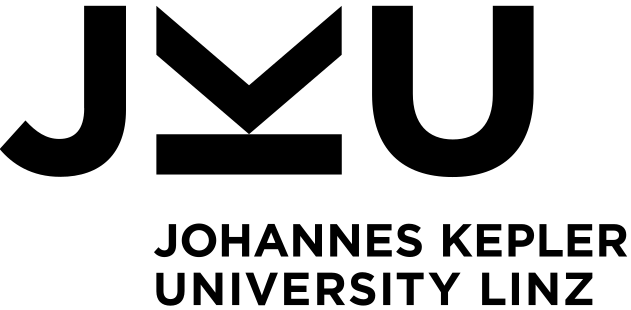
\includegraphics[width=3cm]{jkuen.png}}
	%\else	\ohead*{
\includegraphics[width=3cm]{jkude.png}}
	%\fi
	%\ifoot*{\date}
	%\cfoot*{\name}
	%\ofoot*{\pagemark/\pageref{LastPage}}	
	\ofoot*{\pagemark}
	\setkomafont{pageheadfoot}{\sffamily \scriptsize}
	\setkomafont{pagenumber}{\sffamily \scriptsize}

	\usepackage[onehalfspacing]{setspace}
	
	\usepackage{pdfpages}

	%\usepackage{tabularx}
	%\usepackage{ltxtable}
	%\usepackage{booktabs}
	%\usepackage{rotating}
	%\usepackage{colortbl}
	%\usepackage{multirow}
	
	%\usepackage{xcolor}

	%\usepackage{graphicx}
	%\usepackage{wrapfig}

	\usepackage[section]{placeins} %\FloatBarrier

	\usepackage{float} %[H]

	%\usepackage{enumitem}
		
	%\usepackage{subfiles}
	
%	\usepackage[toc,lof,lot]{multitoc}

\usepackage[
		bookmarksnumbered=true,
		pdfborder={0 0 0},
		pdfa,
		pdftitle={\\pdfTitle},
		pdfauthor={\pdfAuthor},
		pdfsubject={\pdfSubject},
		pdfkeywords={\pdfKeywords}
	]{hyperref}
	
%	\setcounter{tocdepth}{3} %subsubsection
%	\setcounter{secnumdepth}{3}
		
	\tolerance=100
	\clubpenalty=10000
	\widowpenalty=10000
	\displaywidowpenalty=10000
	
%	\addtocontents{toc}{\protect\enlargethispage{2\normalbaselineskip}}
%	\addtocontents{lof}{\protect\enlargethispage{2\normalbaselineskip}}
%	\addtocontents{lot}{\protect\enlargethispage{2\normalbaselineskip}}
	
	\addtokomafont{caption}{\small}
	\setkomafont{captionlabel}{\small\sffamily\bfseries}
	

%%%%%%%%%%%%%%%%%%%%%%%%%%%%%%%%%%%%%%%%%%%%%%%%%%%%%%%%%%%%%%%%%%%%%%%%%%%%%%%%%%%%%%


% Fonts and typesetting
%\setmainfont{tex-gyre-pagella}
%\setmainfont{Tex Gyre Termes}
%\setsansfont{Verdana}
%\setmainfont{Arial}

\newcommand{\mf}[1]{\text{\texttt{#1}}}

\newcommand{\logicRule}[3]{
  \ifstrempty{#1}
  {
    \ifstrempty{#3}
    {
      \[#2\]
    }
    {
      \[\tag*{[#3]} #2\]
    }
  }
  {
    \ifstrempty{#3}
    {
      \[\dfrac{#1}{#2}\]
    }
    {
      \[\tag*{[#3]} \dfrac{#1}{#2}\]
    }
  }
  
}

\newcommand{\semantic}[1]{\llbracket \text{\footnotesize\texttt{#1}} \rrbracket}

\newenvironment{letIn}
{Let}
{\newline
\text{\textemdash}
}


\def\dotsign{\xleaders\hbox to .2em{\d{}}\hfill\d{}}